% Created 2018-05-17 Thu 12:07
% Intended LaTeX compiler: pdflatex
\documentclass[11pt]{article}
\usepackage[utf8]{inputenc}
\usepackage[T1]{fontenc}
\usepackage{graphicx}
\usepackage{grffile}
\usepackage{longtable}
\usepackage{wrapfig}
\usepackage{rotating}
\usepackage[normalem]{ulem}
\usepackage{amsmath}
\usepackage{textcomp}
\usepackage{amssymb}
\usepackage{capt-of}
\usepackage{hyperref}
\usepackage{color}
\usepackage{minted}
\usepackage{color}
\usepackage{minted}
\usepackage{parskip}
\usepackage{geometry}
\usepackage[hang,footnotesize,bf,sf]{subfigure}
\usepackage{caption}
\usepackage[dvipsnames]{xcolor}
\geometry{left=2.5cm,right=2.5cm,top=2.5cm,bottom=2.5cm}
\usepackage{booktabs} \usepackage{tabularx}
\usepackage{tikz} \usetikzlibrary{mindmap,calc,trees,positioning,arrows,chains,shapes.geometric,decorations.pathreplacing,decorations.pathmorphing,shapes,matrix,shapes.symbols,plotmarks,decorations.markings,shadows}
\usepackage{tikz-qtree}
\usepackage{colortbl} 
% \usepackage[table]{xcolor}
\usepackage{qcircuit}

% new command to add annotations (here from Gian)
% all notes cna be eliminated by changing the command to: "\def\noteGG#1{}"
\def\noteGG#1{\textbf{\color{red}[GG: #1]}}
\def\noteLL#1{\textbf{\color{blue}[LL: #1]}}
\def\noteD#1{\textbf{\color{magenta}[D: #1]}}

\author{Daniel Moreno Manzano, Lingling Lao, Carmen G. Almudever}
\date{\today}
\title{Constraints of the Surface-7 and -17 chips}
\hypersetup{
 pdfauthor={Daniel Moreno Manzano},
 pdftitle={Constraints of the Surface chips 7 and 17},
 pdfkeywords={},
 pdfsubject={},
 pdfcreator={Emacs 25.1.1 (Org mode 9.0.5)}, 
 pdflang={English}}
\begin{document}

\maketitle
%\begin{abstract}


In this document the constraints for superconducting quantum processors (Surface-7 and Surface-17) developed at QuTech by Di Carlo's group are summarized. 



\section{Superconducting quantum processor architecture}
\label{sec:topology}

%The term topology refers to how the qubtis are arranged in the quantum chip. 
Figures \ref{Surface17}  and \ref{Surafce17b}, and \ref{fig:org08ec89a}  show the layout of Surface-17 (SC-17) and Surface-7 (SC-7) chips, respectively \cite{versluis2016scalable}. Circles represent qubits and the different colors represent the frequencies for single-qubit microwave control.

Figure \ref{cell} shows the basic unit cell that is composed by 8 qubits. By repeating this unit a surface code can be composed as shown in Figure \ref{SC17}. 

Figure \ref{fig:sc_17} shows a schematic of the layout for the Surface-17 chip \cite{versluis2016scalable}. Every qubit has a dedicated flux-control line (yellow), microwave-drive line (red), and readout resonator (purple). Only qubits connected by bus resonators (in orange) can interact. Diagonal blue lines are feedlines for measurement of qubits. Note that readout resonators are simultaneously interrogated using frequency-division multiplexing. For more details, read \cite{versluis2016scalable,versluis2017scalable}. 


Figures \ref{fig:simple_sc_17} and \ref{fig:org08ec89a}  show a schematic of the topology for both quantum chips, Surface-17 and Surface-7 respectively. Circles represent the \textbf{qubits}  and the \textbf{edges} represent the `connections' between them or possible interactions. Numbers  are the physical addresses of the qubit. As we just mentioned the different colors represent the frequency for single-qubit microwave control: red for $f_1$, blue and green for $f_2$ and pink for $f_3$. \textbf{Note that in this particular case only 3 frequencies are used but 4 different frequencies are also possible}.%The numbers along the direct edges are addresses of the allowed qubit pairs.


\begin{figure}[h!]
\centerline{\subfigure[]{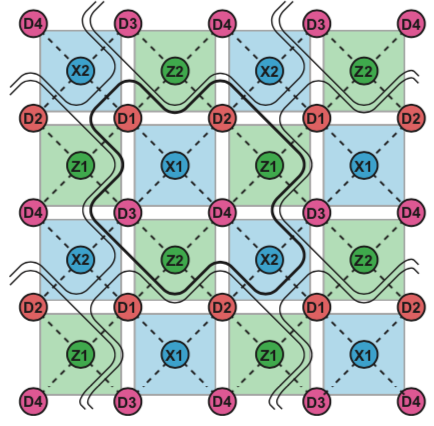
\includegraphics[width=2.5in]{cell}
\label{cell}}
\subfigure[]{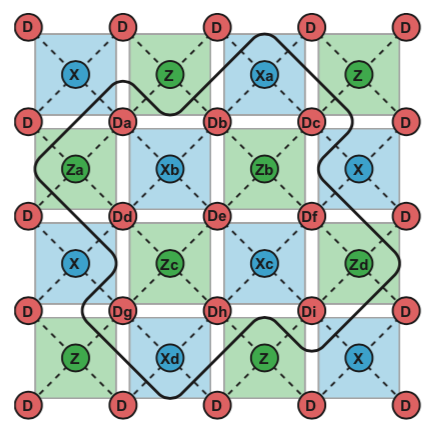
\includegraphics[width=2.5in]{SC_17.png}
\label{SC17}}}
\caption{(a) 8 qubit unit cells that can form a surface code just by repeating them. (b) Surface-17 cell.}
\label{Surface17}
\end{figure}




\begin{figure}[h!]
\centerline{\subfigure[]{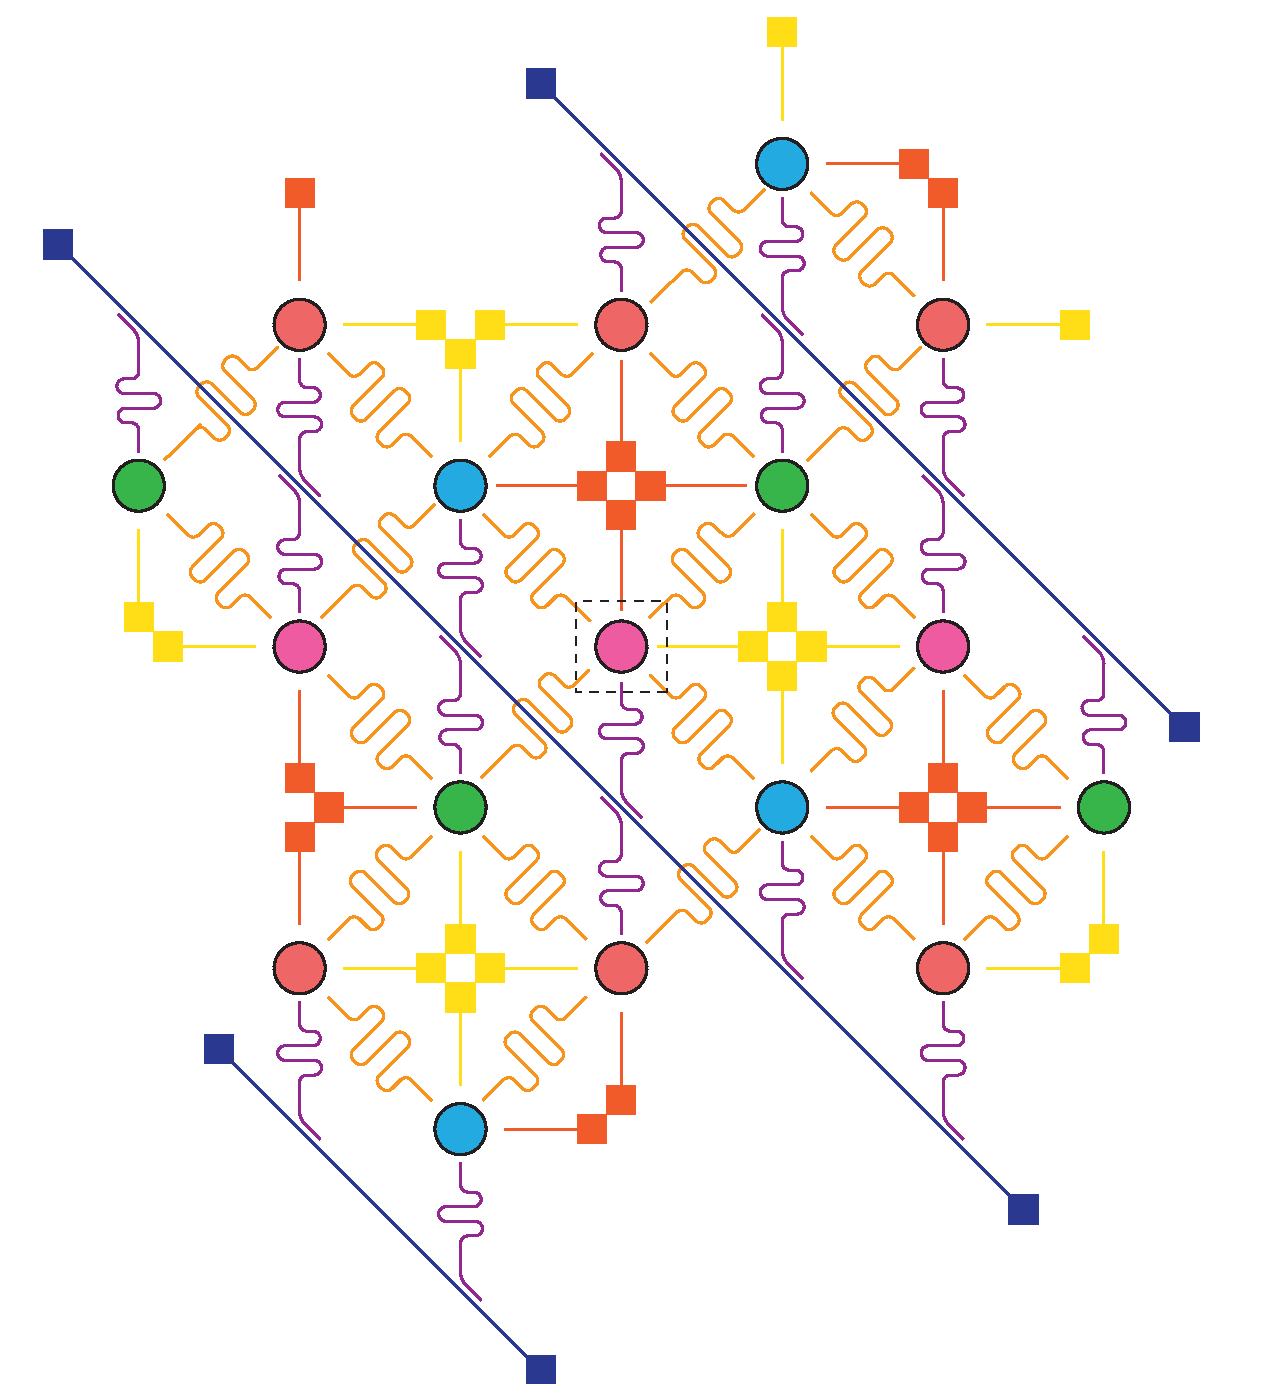
\includegraphics[width=3in]{sc-17}
\label{fig:sc_17}}
\subfigure[]{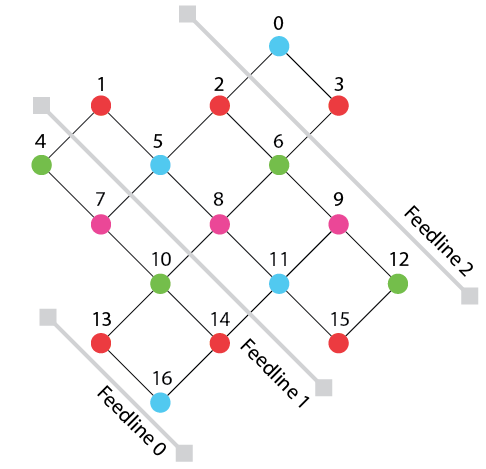
\includegraphics[width=3.5in]{SClayout}
\label{fig:simple_sc_17}}}
\caption{(a) Schematic of the realization of SC-17 chip. (b) Simpler layout of the SC-17. All the examples will refer to this picture}
\label{Surafce17b}
\end{figure}



\begin{figure}[h!]
\centering
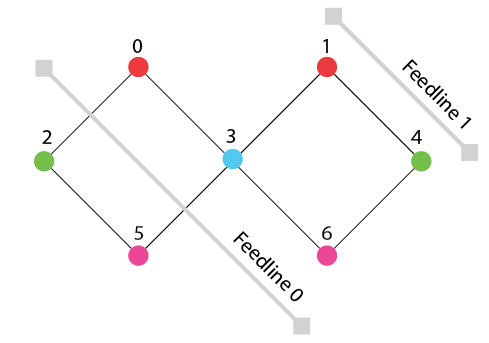
\includegraphics[width=0.5\textwidth]{sc7_w_feedlines.png}
\caption{\label{fig:org08ec89a}
Surface code-7 qubits (SC-7) simplified layout.}
\end{figure}



%In the SC-7 the connections are characterized as the black lines while in the SC-17 are illustrated as the orange waves.
%As one may predict, this will lead us to one of the main constraints, the \emph{nearest neighbors} restriction.


\newpage

\section{Gate set, gate time and gate fidelity}
\label{sec:orgd576c64}


In principle, any kind of single qubit rotation can be performed on the superconducting quantum processor. However, gates need to be calibrated before performing any experiment and obviously one cannot calibrate infinite amount of gates. Furthermore, Z rotations do not perform very well on transmons. Based on these observations, we will limit single qubit gates to X and Y rotations, in which the most common are  $\pm$ 90 (degrees) and $\pm$ 180. Conditional-phase (CZ) gates and measurement in the Z basis are also possible in transmons. Therefore, the gates supported (elementary gates) by the superconducting quantum processor are:

\begin{itemize}
\item X gate with arbitrary angle rotation. Most common  \(\pm 90\) and \(\pm180\) degrees rotations
\item Y gate with arbitrary angle rotation. Most common  \(\pm 90\) and \(\pm180\) degrees rotations
%\item Z gate with arbitrary rotations (error rate < 0.1\%)
\item CZ gate 
\item Measurement in the Z basis ($M_{z}$)
\end{itemize}

Table \ref{primitive_gate_time} shows the gate time and the errors rates for single-qubit gates, CZ gate and measurement \cite{versluis2016scalable}. Note that the default basis of measurement will be Z basis unless one specifies.

\begin{table}[h!]
\centering
\caption{The gate time and fidelity of primitive set from experiments. The measurement time includes both measuring and depletion time.}
\label{primitive_gate_time}
\begin{tabular}{lll}
\textbf{Gate type}    & \textbf{Gate time} & \textbf{Fidelity}       \\
\hline\hline
Single-qubit & 20 ns     &  $\sim 99.97 \%$ \\
\hline

CZ           & 40 ns     & $\sim 99.93 \%$           \\
\hline
$M_{z}$  & 600 ns    & $\sim 99.5 \%$     \\  
\hline
\end{tabular}
\end{table}

In order to perform a single-qubit gate microwave pulses are used whereas flux-pulses (qubit specific detuning sequence) are used for two-qubit gates (CZ). 
For the mapping process, we assume that arbitrary rotations and multi-qubit gates are first decomposed to the Clifford+T group, \{H,T,S,CNOT\}. Although this is a universal gate set that is not directly supported by the quantum chip. 
These gates need to be further decomposed into the elementary gates as shown in Figure \ref{fig:decompositions} and their gate time is shown in Table \ref{uni_set_gatetime}.
%\textcolor{red}{We still need to include SWAP decomposition}


  \begin{figure}[t!]     
\begin{center}
%\resizebox{\textwidth}{!}{%

\begin{minipage}{\textwidth}
\Qcircuit @C=1em @R=.7em {
& \gate{Z} & \qw & \push{\equiv} &  & \gate{X} & \gate{Y} & \qw \\
}
\end{minipage}

\vspace{1cm}

\begin{minipage}{\textwidth}
\Qcircuit @C=1em @R=.7em {
    & \gate{H} & \qw & \push{\equiv} & & \gate{Y_{\text{-90}}} & \gate{Z} & \qw & \push{\equiv} & & \gate{Z} & \gate{Y_{\text{+90}}} & \qw & \push{\equiv} & & \gate{X} & \gate{Y_{\text{-90}}} & \qw\\
}
\end{minipage}     

\vspace{1cm}

\begin{minipage}{\textwidth}
\Qcircuit @C=1em @R=.7em {
& \gate{T} & \qw & \push{\equiv} &  & \gate{H} & \gate{X_{+45}} & \gate{H} & \qw & \push{\equiv} &  & \gate{Y_{\text{+90}}} & \gate{X_{+45}} & \gate{Y_{\text{-90}}} & \qw \\
}
\end{minipage}

\vspace{1cm}

\begin{minipage}{\textwidth}
\Qcircuit @C=1em @R=.7em {
& \gate{T^{\dagger}} & \qw & \push{\equiv} &  & \gate{H} & \gate{X_{-45}} & \gate{H} & \qw & \push{\equiv} &  & \gate{Y_{\text{+90}}} & \gate{X_{-45}} & \gate{Y_{\text{-90}}} & \qw \\
}
\end{minipage}

\vspace{1cm}

\begin{minipage}{\textwidth}
\Qcircuit @C=1em @R=.7em {
& \gate{S} & \qw & \push{\equiv} &  & \gate{H} & \gate{X_{+90}} & \gate{H} & \qw & \push{\equiv} &  & \gate{Y_{\text{+90}}} & \gate{X_{+90}} & \gate{Y_{\text{-90}}} & \qw \\
}
\end{minipage}

\vspace{1cm}

\begin{minipage}{\textwidth}
\Qcircuit @C=1em @R=.7em {
& \gate{S^\dagger} & \qw & \push{\equiv} &  & \gate{H} & \gate{X_{+90}} & \gate{H} & \qw & \push{\equiv} &  & \gate{Y_{\text{+90}}} & \gate{X_{-90}} & \gate{Y_{\text{-90}}} & \qw \\
}
\end{minipage}

\vspace{1cm}

%\begin{minipage}{\textwidth}
%\Qcircuit @C=1em @R=.7em {
% & \ctrl{1} & \qw & \push{\equiv} &  & \qw & \ctrl{1} & \qw & \qw & \push{\equiv} &  & \qw & \qw & \ctrl{1} & \qw & \qw & \qw\\
% & \targ & \qw &  &  & \gate{H} & \control \qw & \gate{H} & \qw &  &  & \gate{Y_{\text{-90}}} & \gate{X} & \control \qw & \gate{Y_{\text{-90}}} & \gate{X} & \qw\\
% }
% \end{minipage}

\begin{minipage}{\textwidth}
\Qcircuit @C=1em @R=.7em {
 & \ctrl{1} & \qw & \push{\equiv} &  & \qw & \ctrl{1} & \qw & \qw \\
 & \targ & \qw &  &  & \gate{Y_{-90}} & \control \qw & \gate{Y_{+90}} & \qw\\
 }
 \end{minipage}
 
 \vspace{1cm}
\begin{minipage}{\textwidth}
\Qcircuit @C=1em @R=.7em {
 & \qswap & \qw  & \push{\equiv}& &\ctrl{1} &\targ & \ctrl{1}&\qw &\push{\equiv}& &\qw&\ctrl{1}&\gate{Y_{-90}}&\control \qw&\gate{Y_{+90}}&\ctrl{1}&\qw&\qw\\
 & \qswap \qwx& \qw & & & \targ &\ctrl{-1}& \targ&\qw& & & \gate{Y_{-90}} &\control \qw&\gate{Y_{+90}}&\ctrl{-1}&\gate{Y_{-90}} &\control \qw&\gate{Y_{+90}}& \qw\\
 }
 \end{minipage}
%}

\end{center}

\caption{Decomposition in the X-Y-Z-CZ set of the Clifford + T gates that are not directly supported in the quantum chip}
\label{fig:decompositions}


\end{figure}


\begin{table}[bth!]
\centering
\caption{The gate time for the universal set \{H,S,T,CNOT\}.} 
\label{uni_set_gatetime}
\begin{tabular}{c|c}
\hline
Gate type & Gate time \\ \hline
X         & 20 ns     \\ 
Y         & 20 ns     \\ 
Z         & 40 ns     \\ 
H         & 40 ns     \\ 
S/Sdag    & 60 ns          \\ 
T/Tdag    & 60 ns          \\ 
CNOT      & 80 ns     \\ 
SWAP      & 200 ns    \\ 
$M_{Z}$         &  600 ns          \\ \hline
\end{tabular}
\end{table}

\begin{table}[bth!]
\centering
\caption{The gate time for the universal set allowed in the devices $\{R_{X},R_{Y},CZ,M_{Z}\}$}.
\label{sc_set_gatetime}
\begin{tabular}{c|c}
\hline
Gate type & Gate time \\ \hline
$R_{X}(\pm 45, \pm90)$         & 20 ns     \\ 
$R_{Y}(\pm 45, \pm90)$       & 20 ns     \\ 
CZ        & 40 ns     \\ 
$M_{Z}$         &  600 ns          \\ \hline
\end{tabular}
\end{table}

%\newpage
In the next sections, the different constraints of the superconducting quantum chip will be explained in detail. Note that we will distinguish two kind of constraints: the ones coming from the quantum chip- e.g. nearest-neighbour interactions- that we call \textbf{hardware constraints} and the ones from the electronics control setup - e.g. qubits operated by the same AWG- called \textbf{electronics constraints}. In addition, we will also make a distinction between \textbf{hard} and \textbf{soft} constraints. \textbf{Hard} constraints are those that will remain there and will hardly change and \textbf{soft} constraints are those that will be evolving, changing and even disappearing at some point. 






\section{Qubits interaction constraint (Hard)}
\label{sec:org77a3a48}

As shown in the previous section, qubits are not fully `connected'.
In Surface-7 and Surface-17 each qubit is connected to a maximum of four qubits, the nearest-neighbours, limiting the possible interactions -e.g. two-qubit gate- between them (hardware constraint). This constraint will make that qubits that need to interact and are not place in neighboring positions will need to be moved to adjacent positions. Quantum states in superconducting technology can be `moved' by using SWAP operations.


%It is the origin of the mapping problem.
%Therefore, a mapping pass that  is required to run any quantum algorithm in a physical device.




This constraint implies that in Surface-17





% \linebreak[4]
\begin{minipage}[t]{.45\textwidth}

It is possible to do:

\begin{minted}[frame=lines,fontsize=\scriptsize,linenos,breaklines,breakanywhere]{c}
CZ q[1],q[5]
CZ q[8],q[6]
CZ 1Figure\end{minted}

\end{minipage}
\hfill %\hspace{1cm}
\begin{minipage}[t]{.45\textwidth}

but impossible to do (directly, without any mapping):

\begin{minted}[frame=lines,fontsize=\scriptsize,linenos,breaklines,breakanywhere]{c}
CZ q[1],q[2]
CZ q[0],q[16]
\end{minted}

\end{minipage}

The code shown here and in the next sections is written in an eQASM fashion.
The letters represent the kind of gate operation and the number will refer to the qubit number in the Surface-17 layout (Figure \ref{fig:simple_sc_17}).
Also, the character '\texttt{|}' represents the operations that can be executed in parallel. 



% \section{Dependency operation constraint (Hard)}

% \label{sec:org73a281f}

% Qubits can be, exclusively, in one of the following states:

% \begin{itemize}
% \item Idling
% \item Being used in a single- or multi-qubit gate
% \item Being measured
% \end{itemize}

% \begin{minipage}[t]{.45\textwidth}

% Then,

% It is possible to do:

% \begin{minted}[frame=lines,fontsize=\scriptsize,linenos,breaklines,breakanywhere]{c}
% X 1
% Y 1
% \end{minted}

% \end{minipage}
% \hfill %\hspace{1cm}
% \begin{minipage}[t]{.45\textwidth}

% but not:

% \begin{minted}[frame=lines,fontsize=\scriptsize,linenos,breaklines,breakanywhere]{c}
% X 1 | Y 1
% \end{minted}

% \end{minipage}

% This constraint will affect the scheduling of operation, as there is a dependency between gates.

\section{Frequency constraint (Soft)}
\label{sec:orgff4c391}

\subsection{Single-qubit gates}

In order to perform single-qubit gates, electromagnetic microwaves are sent. As shown in Figures \ref{fig:simple_sc_17} and \ref{fig:org08ec89a}, three or four different frequencies for single-qubit microwave control can be used in Surface-7 and Surface-17. In principle, any qubit can be operated individually and then any combination of single-qubit gates can be performed in parallel. However, qubits using the same frequency are controlled by the same QWG and then limiting the possible parallelism of operations (control electronics constraint). We can then group qubits in 3 or 4 groups for SC-7 and SC-17 as shown in the following tables.




\begin{table}[h!]


\caption{\label{T1}
Frequency groups for Surface-7 when using 3 different frequencies. }
\centering

\begin{tabular}{lll}
 & \\
\hline
QWG & Qubits & Frequency group\\
\hline
\cellcolor{red!25}  0 & \cellcolor{red!25} 0, 1 & \cellcolor{red!25} $f_1$\\
\cellcolor{Aquamarine!25}  1 & \cellcolor{Aquamarine!25} 2, 3, 4 & \cellcolor{Aquamarine!25} $f_2$\\
\cellcolor{pink!25}  2 & \cellcolor{pink!25} 5, 6 & \cellcolor{pink!25} $f_3$\\

\hline
\end{tabular}
%\end{minipage}
\end{table}

 
 \begin{table}[h!]


\caption{\label{T2}
Frequency groups for Surface-7 when using 4 different frequencies.}
\centering
\begin{tabular}{lll}
 & \\
\hline
QWG & Qubits & Frequency Group\\
\hline
\cellcolor{red!25}  0 & \cellcolor{red!25} 0, 1 & \cellcolor{red!25} $f_1$ \\
\cellcolor{pink!25}  1 & \cellcolor{pink!25} 5, 6 & \cellcolor{pink!25} $f_3$ \\
\cellcolor{green!25}  2 & \cellcolor{green!25} 2, 4 & \cellcolor{green!25} $f_2$ \\
\cellcolor{cyan!25}  3 & \cellcolor{cyan!25} 3 & \cellcolor{cyan!25} $f_2$ \\
\hline
\end{tabular}
\end{table}
 
 
 





\begin{table}[h!]

\caption{\label{T4}
Frequency groups for Surface-17 when using 3 different frequencies.}
\centering
\begin{tabular}{lll}
 & \\
\hline
QWG & Qubits & Frequency Group\\
\hline
\cellcolor{red!25}  0 & \cellcolor{red!25} 1, 2, 3, 13, 14, 15 & \cellcolor{red!25} $f_1$\\
\cellcolor{pink!25}  1 & \cellcolor{pink!25} 7, 8, 9 & \cellcolor{pink!25} $f_3$\\
\cellcolor{Aquamarine!25}  2 & \cellcolor{Aquamarine!25} 0, 4, 5, 6, 10, 11, 12 16 & \cellcolor{Aquamarine!25} $f_2$\\
\hline
\end{tabular}
\end{table}
%\end{minipage}


\begin{table}[h!]


\caption{\label{T3}
Frequency groups for Surface-17 when using 4 different frequencies.}
\centering
\begin{tabular}{lll}
 & \\
\hline
QWG & Qubits & Frequency Group\\
\hline
\cellcolor{red!25}  0 & \cellcolor{red!25} 1, 2, 3, 13, 14, 15 & \cellcolor{red!25} $f_1$\\
\cellcolor{pink!25}  1 & \cellcolor{pink!25} 7, 8, 9 & \cellcolor{pink!25} $f_3$\\
\cellcolor{green!25}  2 & \cellcolor{green!25} 4, 6, 10, 12 & \cellcolor{green!25} $f_2$\\
\cellcolor{cyan!25}  3 & \cellcolor{cyan!25} 0, 5, 11, 16 & \cellcolor{cyan!25} $f_2$\\
\hline
\end{tabular}
\end{table}


\newpage
It is not possible to perform two different single-qubit gates at the same time on qubits using the same frequency (same color, connected to the same QWG). For instance in SC-17,

\begin{minipage}[t]{.45\textwidth}

It is possible to do:

\begin{minted}[frame=lines,fontsize=\scriptsize,linenos,breaklines,breakanywhere]{c}
{ X q[1] | X q[7] }
{ X q[6] | Y q[7] }
{ X q[1] | X q[2] | X q[5] | X q[0] }
{ Y q[10] | Y q[4] }

\end{minted}

\end{minipage}
\hfill %\hspace{1cm}
\begin{minipage}[t]{.45\textwidth}

But not

\begin{minted}[frame=lines,fontsize=\scriptsize,linenos,breaklines,breakanywhere]{c}
{ X q[1] | Y q[2] }
{ X q[5] | Y q[0] }
{ X q[10] | Y q[4] }
{ X q[7] | Y q[9] }
\end{minted}

\end{minipage}

Obviously, it is not possible to perform more than one single-qubit gate on the same qubit at the same time (gate dependency).

\subsection{Two-qubit gates}

In order to perform a two quibt gate in transmons, interacting qubits need to be brought to a specific close frequencies \cite{versluis2016scalable}. More specifically, $CZ_f$ gates are performed between qubits at $f^{int}_1$ and $f_2$ or at $f^{int}_2$ and $f_3$ as shown in Figure \ref{detuning}. This limits the amount of two-qubit gates that can be performed in parallel (hardware constraint). In addition, note that, different frequency arrangements can be used as shown in Figure \ref{sequence}. 


\begin{figure}[h!]
\centerline{\subfigure[]{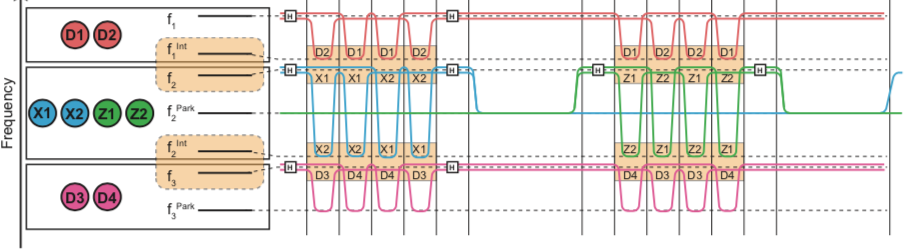
\includegraphics[width=5in]{detuning.png}
\label{detuning}}
\subfigure[]{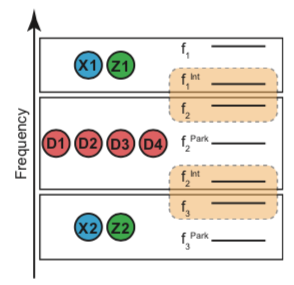
\includegraphics[width=1.5in]{Frequencies.png}
\label{freq}}}
\caption{(a) Frequency arrangement and detuning frequencies for the qubits in the unit cell. (b) Alternative frequency arrangement for qubits in the unit cell.}
\label{sequence}
\end{figure}


Based on the unit cell in Figure \ref{cell} and assuming the frequency scheme of Figure \ref{detuning} we can formulate the following: 1) If a two-qubit gate is being performed between D1 (D2) and X1 (X1 or Z1), D2 (D1) cannot interact with X1 or Z1 (X1) at the same time; 2) In the same way, if a two-qubit gate is being performed between D3 (D4) and X1 or Z2 (X1 or Z1 or X2 or Z2), D4 (D3) cannot interact with X1 or Z1 or X2 or Z2 (X1 or Z2) at the same time. Obviously,  if a two-qubit gate is being performed between two qubits, the qubits involved can not perform another single- or two-qubit gate at the same time. A summary of the gates that can or cannot be performed in paralallel is shown in Table \ref{parallelCZ}.

\begin{table}[h!]
\centering
\caption{Allowed and not allowed parallel CZ gates in the unit cell.}
\label{parallelCZ}
\small
\resizebox{0.80\textwidth}{!}{
\begin{tabular}{|c|c|c|}
\hline
CZ gate    & NOT Possible gates in parallel                  & NOT Possible single-qubit gates   \\ \hline
D1-X1      & D2-X1, D3-X1, D4-X1, D2-Z1                      &  X2, D1, X1\\ \hline
D2-X1      & D1-X1, D3-X1, D4-X1, D2-Z1                      &  X2, D2, X1 \\ \hline
D3-X1      & D1-X1, D2-X1, D4-X1, D3-Z2, D4-Z1, D4-Z2, D4-X2 &  D4, D3, X1                     \\ \hline
D3-Z2      & D3-X1, D4-X1, D4-X2, D4-Z1, D4-Z2               &  D4, D3, Z2       \\ \hline
D4-X1      & D1-X1, D2-X1, D3-X1, D4-Z1, D4-Z2, D4-X2, D3-Z2 &  D3, D4, X1                     \\ \hline
D2-Z1             & D2-X1, D4-Z1, D1-X1                      &  Z2, D2, Z1 \\ \hline
D4-Z2      & D3-X1, D3-Z2, D4-X1, D4-X2, D4-Z1               &  D3, D4, Z2        \\ \hline
D4-Z1      & D3-X1, D3-Z2, D4-X1, D4-X2, D4-Z2, D2-Z1        &  D3, D4, Z1               \\ \hline
D4-X2      & D3-X1, D3-Z2, D4-X1, D4-Z1, D4-Z2               &  D3, D4, X2       \\ \hline

\end{tabular}}
\end{table}


This can be extended to SC-17 based on the same frequency scheme and the simplified layout shown in Figure \ref{fig:simple_sc_17}. \textcolor{red}{We need to derive what operations can be performed in parallel and fill Table \ref{parallelCZSC17} in.}

\textcolor{red}{We also need to derive what operations can be performed in parallel for SC-7.}

\begin{table}[h!]
\caption{Allowed and not allowed parallel CZ gates in SC-17.}
\label{parallelCZSC17}
\centering
\scriptsize
\resizebox{0.80\textwidth}{!}{
\begin{tabular}{|c|c|c|}
\hline
CZ gate & Not possible parallel two-qubit gates & Not allowed qubits for single-qubit gates\\
\hline
Q0-Q2 & Q1-Q5,Q2-Q5,Q2-Q6,Q3-Q0,Q3-Q6 & Q0,Q2,Q5,Q11,Q16\\
\hline
Q0-Q3 & Q0-Q2,Q2-Q6,Q3-Q6,Q2-Q5  & Q0,Q3,Q5,Q11,Q16\\
\hline
Q1-Q4 & Q1-Q5,Q2-Q5,Q4-Q7 & Q1,Q4,Q6,Q10,Q12\\
\hline
Q1-Q5 & Q1-Q4,Q5-Q7,Q2-Q5,Q5-Q8,Q2-Q0,Q2-Q6 & Q1,Q5,Q0,Q11,Q16\\
\hline
Q2-Q5 & Q1-Q4,Q1-Q5,Q2-Q0,Q2-Q6,Q0-Q3,Q3-Q6,Q5-Q7,Q5-Q8 & Q2,Q5,Q0,Q11,Q16\\
\hline
Q2-Q6 & Q1-Q5,Q2-Q5,Q2-Q0,Q6-Q8,Q0-Q3,Q6-Q9,Q3-Q6 & Q2,Q6,Q4,Q10,Q12\\
\hline
Q3-Q6 & Q2-Q5,Q2-Q0,Q2-Q6,Q6-Q8,Q0-Q3,Q6-Q9 & Q3,Q6,Q4,Q10,Q12\\
\hline
Q4-Q7 & Q1-Q4,Q5-Q7,Q7-Q10,Q5-Q8,Q8-Q10 & Q4,Q7,Q8\\
\hline
Q5-Q7 & Q4-Q7,Q1-Q5,Q7-Q10,Q2-Q5,Q5-Q8,Q8-Q10,Q6-Q8,Q8-Q11 & Q5,Q7,Q8\\
\hline
Q5-Q8 & Q4-Q7,Q1-Q5,Q5-Q7,Q7-Q10,Q8-Q10,Q8-Q6,Q8-Q11,Q6-Q9,Q9-Q11 & Q5,Q8,Q7,Q9\\
\hline
Q6-Q8 & Q5-Q7,Q7-Q10,Q5-Q8,Q8-Q10,Q2-Q6,Q8-Q11,Q3-Q6,Q6-Q9,Q9-Q11 & Q6,Q8,Q7,Q9\\
\hline
Q6-Q9 & Q5-Q8,Q8-Q10,Q2-Q6,Q6-Q8,Q8-Q11,Q3-Q6,Q9-Q11,Q9-Q12 & Q6,Q9,Q8\\
\hline
Q7-Q10 & Q4-Q7,Q5-Q7,Q10-Q13,Q5-Q8,Q8-Q10,Q10-Q14,Q6-Q8 ,Q8-Q11  & Q7,Q10,Q8\\
\hline
Q8-Q10 & Q5-Q7,Q7-Q10,Q10-Q13,Q5-Q8,Q10-Q14,Q6-Q8,Q8-Q11,Q6-Q9,Q9-Q11 & Q8,Q10,Q7,Q9\\
\hline
Q8-Q11 & Q5-Q7,Q7-Q10,Q5-Q8,Q8-Q10,Q6-Q8,Q11-Q14,Q6-Q9,Q9-Q11,Q11-Q15,Q9-Q12  & Q8,Q11,Q7,Q9\\
\hline
Q9-Q11 & Q5-Q8,Q8-Q10,Q6-Q8,Q8-Q11,Q11-Q14,Q6-Q9,Q11-Q15,Q9-Q12 & Q9,Q11,Q8\\
\hline
Q9-Q12 & Q6-Q8,Q8-Q11,Q6-Q9,Q9-Q11,Q12-Q15 & Q9,Q12,Q8\\
\hline
Q10-Q13 & Q7-Q10,Q13-Q16,Q8-Q10,Q10-Q14,Q14-Q10,Q11-Q14 & Q10,Q13,Q4,Q6,Q12\\
\hline
Q10-Q14 & Q7-Q10,Q10-Q13,Q13-Q16,Q8-Q10,Q14-Q16,Q11-Q14,Q11-Q15 & Q10,Q14,Q4,Q6,Q12\\
\hline
Q11-Q14 & Q10-Q13,Q13-Q16,Q10-Q14,Q14-Q16,Q8-Q11,Q9-Q11,Q11-Q15,Q12-Q15 & Q11,Q14,Q5,Q0,Q16\\
\hline
Q11-Q15 & Q10-Q14,Q14-Q16,Q8-Q11,Q11-Q14,Q9-Q11,Q12-Q15 & Q11,Q15,Q5,Q0,Q16\\
\hline
Q12-Q15 & Q11-Q14,Q11-Q15,Q9-Q12 & Q12,Q15,Q4,Q6,Q10\\
\hline
Q13-Q16 & Q10-Q13,Q10-Q14,Q14-Q16,Q11-Q14  & Q13,Q16,Q0,Q11,Q5\\
\hline
Q14-Q16 & Q10-Q13,Q13-Q16,Q10-Q14,Q11-Q14,Q11-Q15 & Q14,Q16,Q0,Q11,Q5\\
\hline
\end{tabular}
}
\end{table}

\subsection{Summary for single-qubit and two-qubit gates}

\textbf{Single-qubit gates:} for performing a single-qubit gate on a qubit, one needs to send the required electromagnetic microwave to it.  \textbf{The same} single-qubit gate can be performed in parallel in all or some of the qubits connected to the same QWG. However, it is not possible to perform in parallel a different single qubit-gate in qubits connected to the same QWG.

\textbf{Two-qubit gates:} in order to perform a two-qubit gate in transmons, interacting qubits need to be brought to a specific close frequencies. In addition, the qubits that share a connection with the qubits performing a 2-qubit gate need to be detunned away. %% For instance, in SC-17, when performing a CZ(11,14), q16 and q10 need to be detunned to $f_{2}^{park}$. Note that it is not possible to perform a single-qubit gate (in parallel with the two-qubit gate) on the qubits that have been detunned to  $f_{1}^{int}$,  $f_{2}^{park}$, $f_{2}^{int}$ or $f_{3}^{park}$.

As an example, in fig. \ref{fig:two_qubit_gate_ex}, a CZ gate is applied between qubits 11 and 14 (\texttt{cz (q[11], q[14])}). Thus, both qubits need to be tuned to closer frequencies -- $f_1^{int}$ and $f_2$ in this case. And, as explained before, in order to not create intereferences between qubits some of them should be detunned away. Specifically, qubits 10 and 16 need to be detunned to $f_2^{park}$ because they share a connection with the qubits performing the CZ gate. This means that no single-qubit gate can be applied to these qubits that are outside their main frequency ($f_2$). And, also, that they cannot perform another two-qubit gate at the same time with any other qubit from the QWG 0 -- the red qubits with main frequency $f_1$ -- because it is required to tune them to $f_2$.

One may see a similar example with the SC-7 in fig. \ref{fig:two_qubit_gate_ex}. In this case a CZ gate is applied between qubits 0 and 2 (\texttt{cz (q[0], q[2])}). Following the same reasoning, single-qubit gates cannot be executed on qubit 3. Two-qubit gates with qubits from QWG 0 are not allowed, as well. But, in this case, any two-qubit gate with the qubits from QWG 1 -- the pink qubits with main frequency $f_3$ -- is allowed. This is due to qubit 3 is not allowed to be tunned to $f_2$ but it is allowed to be tunned to $f_2^{int}$, closer to $f_3$.

Finally, for both instances in fig. \ref{fig:two_qubit_gate_ex}, all the qubits that are already in use cannot be used at the same time. Therefore, qubits 11 and 14 in the SC-17 example and qubits 0 and 2 in the SC-7 one cannot be used in any single- or two-qubit gates.



\begin{figure}[h!]
\centering
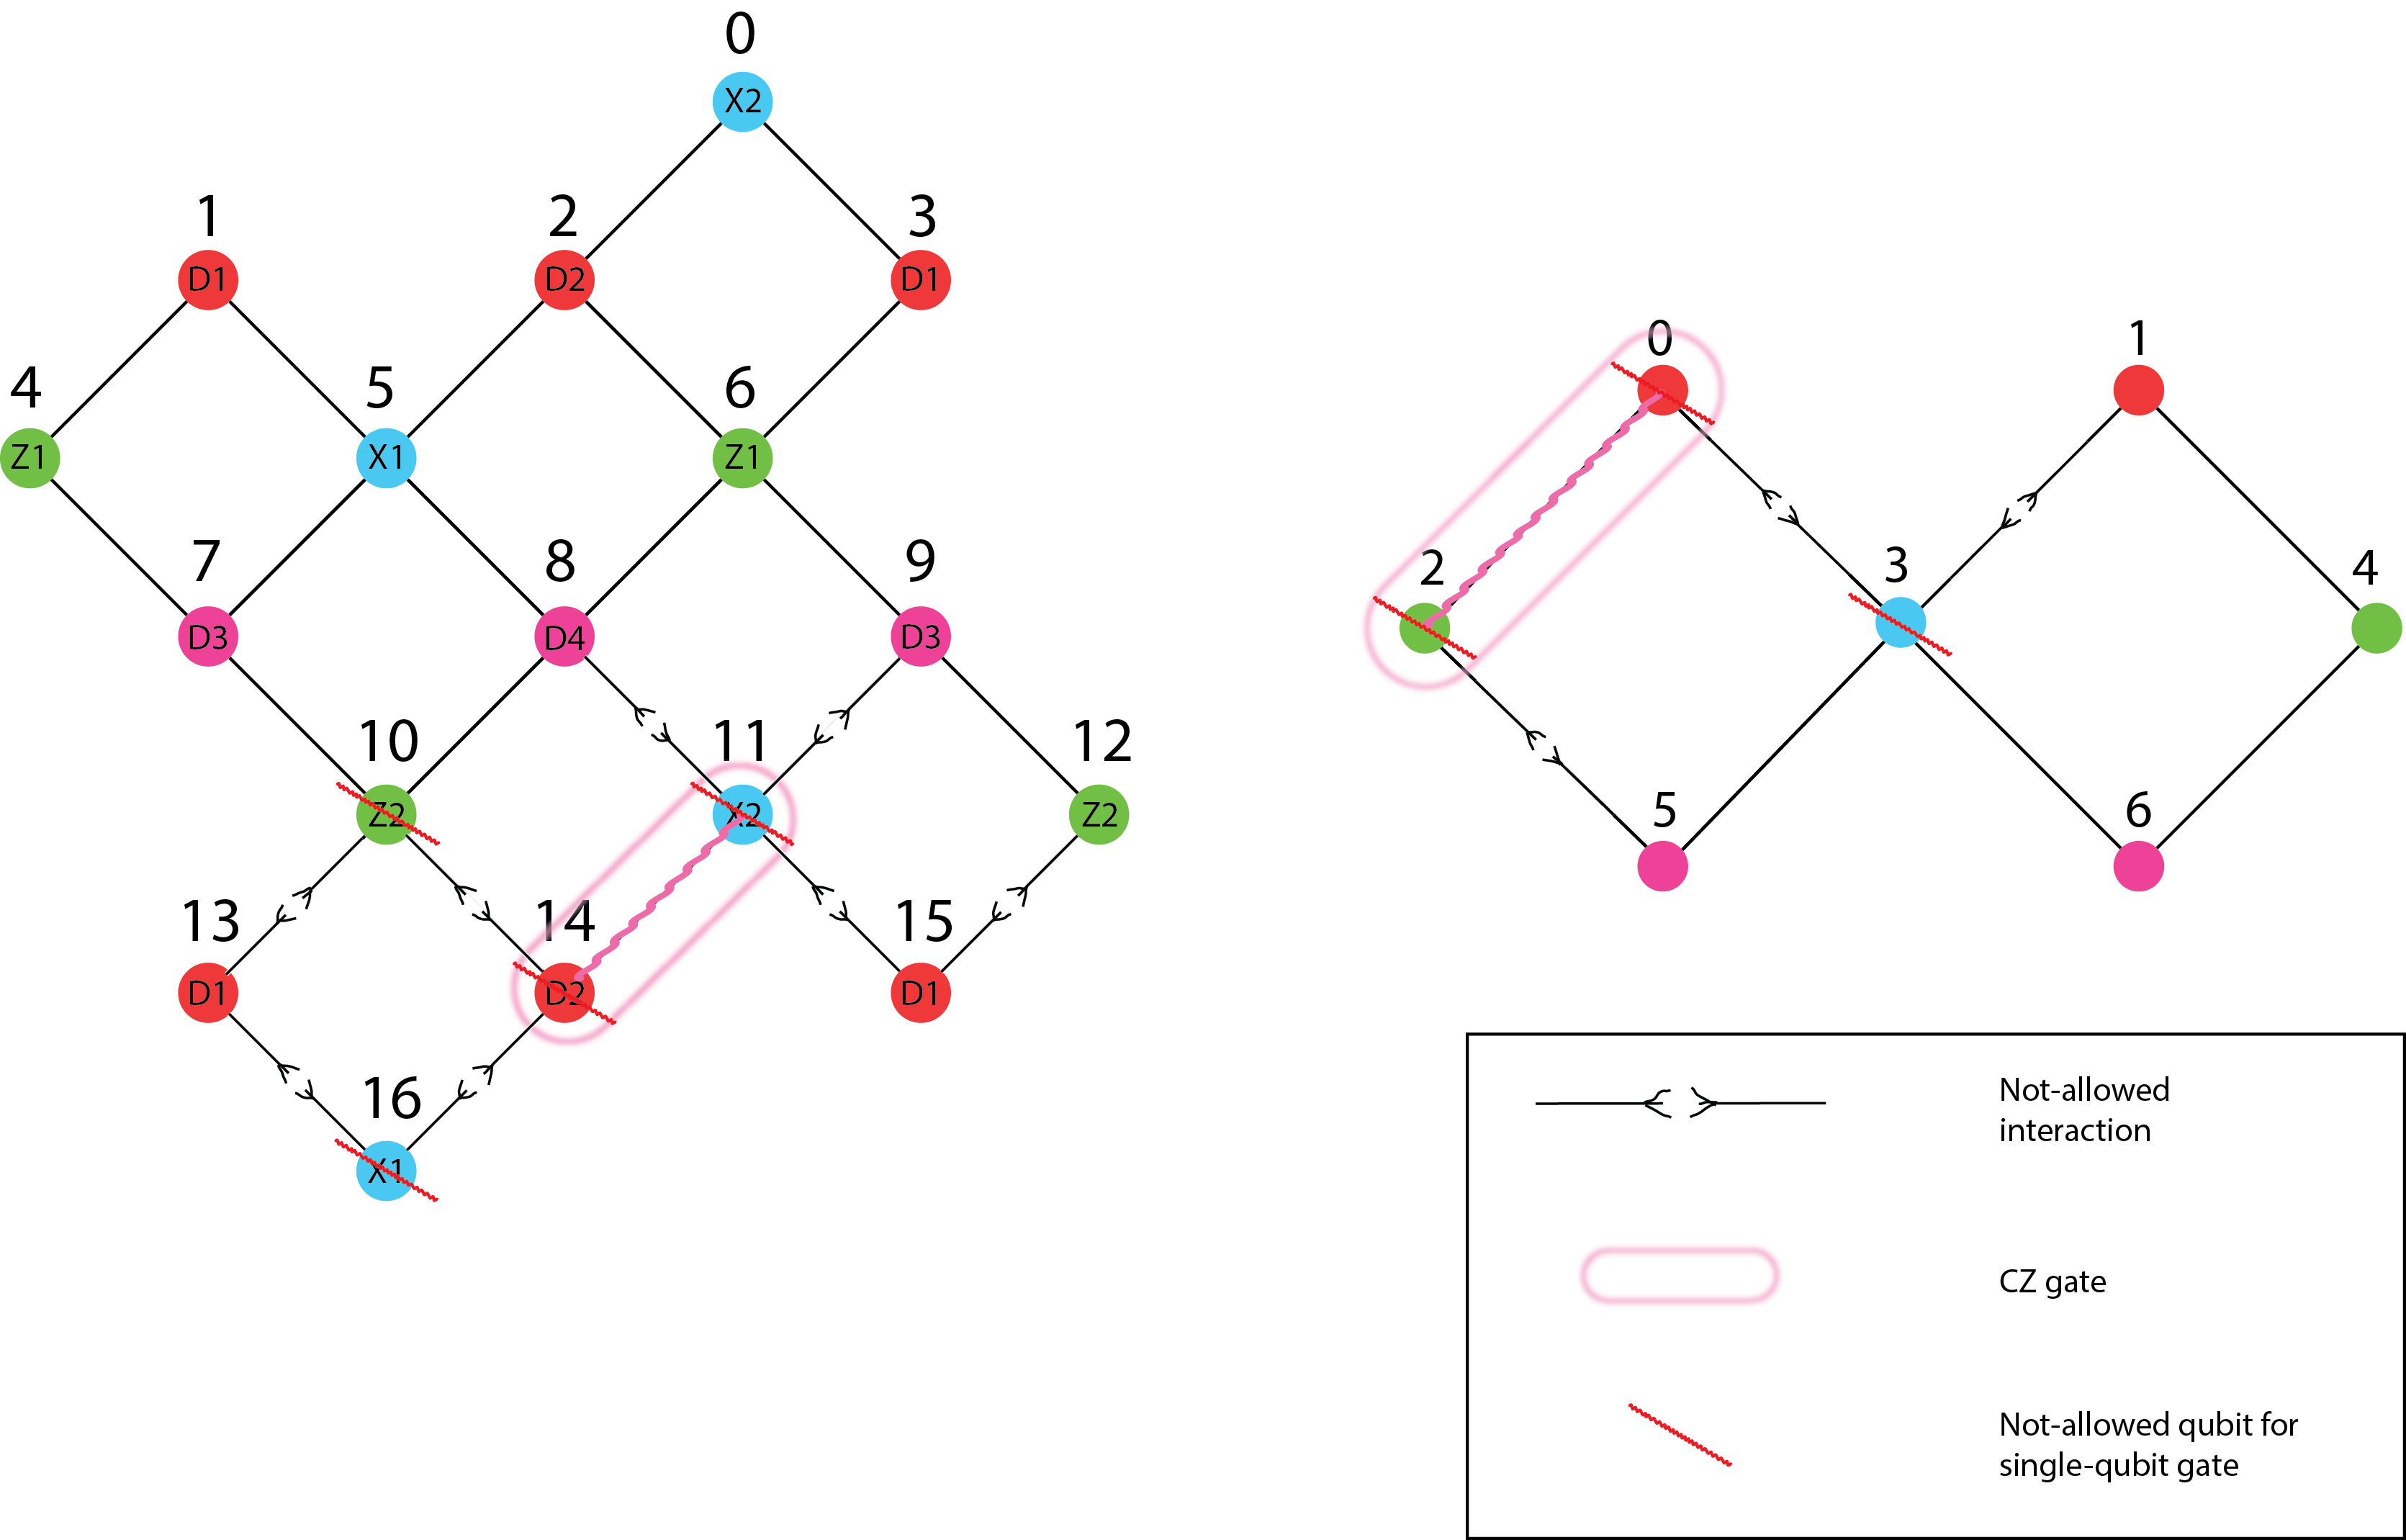
\includegraphics[width=\textwidth]{two_qubit_constraint_sc17.png}
\caption{\label{fig:two_qubit_gate_ex}
Example of a two qubit gate and the consequences of it in SC-17 and SC-7}
\end{figure}

%More specifically, the two next connection in the same axis will be forbidden for two-qubit interactions. The first connection as a consequence of the qubit exclusivity constraint because one of the qubits is being used.
%And the second one is a consequence of this constraint.

%In fig. \ref{fig:mesh} a picture of an infinite qubits mesh is drawn.
%In the example, a two-qubit gate is happening between qubits d and e.
%As a consequence, you can see the closer connections that are forbidden and in green the ones that could be use at the same time.

% \begin{figure}[b!]
     
%      \tikzset{cross/.style={cross out, draw=black, fill=none, minimum size=2*(#1-\pgflinewidth), inner sep=0pt, outer sep=0pt}, cross/.default={5pt}}
     
%      \begin{center}
%      \resizebox{\textwidth}{!}{%

% \begin{tikzpicture}[x=5mm,y=5mm]

% \node [circle,fill=black,minimum size=10pt] at (0,0) {};
% \node [circle,fill=black,minimum size=10pt] at (10,0) {};
% \node [circle,fill=black,minimum size=10pt] at (20,0) {};
% \node [circle,fill=black,minimum size=10pt] at (5,5) {};
% \node [circle,fill=black,minimum size=10pt] at (5,-5) {};
 % \node [circle,fill=black,minimum size=10pt] at (15,5) {};
% \node [circle,fill=black,minimum size=10pt] at (25,5) {};
% \node [circle,fill=black,minimum size=10pt] at (15,-5) {};
% \node [circle,fill=black,minimum size=10pt] at (25,-5) {};
% \node [circle,fill=black,minimum size=10pt] at (30,0) {};

% \node [purple] at (1,0) {\huge a};
% \node [purple] at (11,0) {\huge d};
% \node [purple] at (21,0) {\huge g};
% \node [purple] at (6,5) {\huge b};
% \node [purple] at (16,5) {\huge e};
% \node [purple] at (26,5) {\huge h};
% \node [purple] at (6,-5) {\huge c};
% \node [purple] at (16,-5) {\huge f};
% \node [purple] at (26,-5) {\huge i};
% \node [purple] at (31,0) {\huge j};


% \draw (0,0) -- (5,5) node [midway, above, sloped] {};
% \draw (2.5,2.5) node[cross=5pt,rotate=45,red] {};

% \draw (5,5) -- (10,0)  node [midway, above, sloped] {};
% \draw (7.5,2.5) node[cross=5pt,rotate=45,red] {};

% \draw [line width=0.5mm,cyan] (10,0)  -- (15,5) node [midway, above, sloped] {};

% \draw (15,5) -- (20,0) node [midway, above, sloped] {};
% \draw (17.5,2.5) node[cross,rotate=45,red] {};

% \draw (20,0) -- (25,5) node [midway, above, sloped] {};
% \draw (22.5,2.5) node[cross,rotate=45,red] {};

% \draw [green] (20,0) -- (15, -5) node [midway, above, sloped] {};

% \draw (15, -5) -- (10, 0) node [midway, above, sloped] {};
% \draw (12.5,-2.5) node[cross,rotate=45,red] {};

% \draw (10, 0) -- (5, -5) node [midway, above, sloped] {};
% \draw (7.5,-2.5) node[cross,rotate=45,red] {};

% \draw [green] (5, -5) -- (0,0) node [midway, above, sloped] {};

% \draw [green] (20, 0) -- (25,-5) node [midway, above, sloped] {};
% %\draw (22.5,-2.5) node[cross,rotate=45,red] {};

% \draw [green] (25,5) -- (30,0) node [midway, above, sloped] {};


% \draw [green] (30,0) -- (25,-5) node [midway, above, sloped] {};
% %\draw (27.5,-2.5) node[cross,rotate=45,red] {};

% \draw[dotted] (0,0) -- (-5,5);
% \draw[dotted] (0,0) -- (-5,-5);
% \draw[dotted] (30,0) -- (35,5);
% \draw[dotted] (30,0) -- (35,-5);

% \end{tikzpicture}

%      }
%      \end{center}

%           \caption{Example of the connection constraint in an infinite qubits mesh}
%      \label{fig:mesh}


     
%      \end{figure}



\section{Measurement constraint (Hard)}
\label{sec:org58adcb1}

Measuring the qubits is done by using feedlines coupled to several qubits.
For example, in the SC-17 chip, the feedline 1 is used to measure qubits 1, 4, 5, 7, 8, 10, 11, 14 and 15. This will lead us to the last limitation, the \emph{measurement constraint} (hardware constraint). In this case, the measurement on a qubit cannot start when
another qubit coupled to the same feedline is being measured, but it
allows to start measurement on any combination of qubits coupled to
the same feedline at the same time.  Furthermore, there is no dependency between
measurements of any two qubits coupled to different feedlines.



\begin{minipage}[t]{.45\textwidth}

In SC-17, it is possible to do

\begin{minted}[frame=lines,fontsize=\scriptsize,linenos,breaklines,breakanywhere]{c}
  
measure q[0] | measure q[2] | measure q[3] | measure q[6] | measure q[9] | measure q[12]
measure q[1] | measure q[13]
qwait 30
measure q[3] | measure q[8]

\end{minted}

notice that the measurement of qubits 13 and 16 is executed at the same cycle.     

\end{minipage}
\hfill %\hspace{1cm}
\begin{minipage}[t]{.45\textwidth}

On the other hand it is not possible to do

\begin{minted}[frame=lines,fontsize=\scriptsize,linenos,breaklines,breakanywhere]{c}
  
  measure q[2]
  measure q[6]
  
\end{minted}

Note that, in order to measure qubit 2 and 6 in different times, the latter instruction should wait 30 cycles for the first one to finish. In other words, this code is missing a \texttt{qwait 30} instruction.

\end{minipage}








\bibliography{thesis_plan}
\bibliographystyle{plain}

\section{Mapping models}

\subsection{TU Delft Mapping model: initial placement, routing and scheduling}

\textcolor{red}{Carmina: please add reference to the paper, if any}

\subsection{Gian Giacomo Mapping model}

Initial placement may be: trivial, provided in input, random, or based on the first gate per logical qubit. Routing is base on improving the two-qubit gate pattern, not yet described in a paper or bench marked. Some concepts and techniques are described in \cite{Guerreschi2018}. I have not implemented any reduction of the gates (for example the cancellation of consecutive, opposite rotations or consecutive CZ), but it can be added if present in the other compilers.

\subsection{JK Linz University Mapping model}
\textcolor{red}{Please add reference to the paper, if any}
\newpage

\section{Minutes telco 11/07/2018}

We discussed what benchmarks we will use, what should be the input/output of the mappers and the constraints of 7 and 17 superconducting quantum chips.

\textbf{We agreed on the following:}

\begin{itemize}
    \item The input of the mapping models is a c-QASM file in which gates have been already decomposed to the elementary gates supported by the device. The code is just sequential code (no parallel sections or timing information).
    
    \item The first version of the mapping model will insert SWAPs that will be decomposed and re-schedule afterwards. We will all use the time of 3 CNOTs.
    
    \item The mapping model only take into account the connectivity constraint but it will also use the other constraints if operations are re-schedule and /or it optimizes for latency. 
    
    \end{itemize}



\textbf{Action points:}

\begin{itemize}

    \item Only the OpenQL version of the benchmarks is available in Github. Daniel will generate the c-QASM version and put it on Github. He will let the other know when it is available. He will also look at the distribution of the gates for each benchmark to check if the have a sufficient representation/variety of benchmarks in terms of percentage of 2-qubit gates. From very low to very high.
    
    \item Lingling will look at the decomposition of the SWAP gate.
    
    \item Daniel will check table 6 and fill Table 7 in. We will see if you can observe any patterns that allow us to express what parallel operations are allowed in a more efficient way.
    
    \item Carmina will give access to Gian, Alwin and Robert to the constraints document.
    
    \item We (TU Delft) will double-check the duration for each primitive gate and calculate the duration of the SWAP gate (Lingling). 
    
    \end{itemize}
    
    
    
\begin{table}[!h]
\centering
\scriptsize
\caption{Mapping tasks}
\label{tab:openql-overview}
\begin{minipage}[c]{\linewidth}
\begin{tabular}{llll}
\toprule
Task \# & Task & Responsible  & Status\footnote{\scriptsize Not started/In progress/Complete} \\
\midrule
 1 & Benchmarks in c-QASM                          & Daniel    & Done  \\
 2 & Benchmarks CNOT percentage                    & Daniel         & Done      \\
 3 & SWAP decomposition and gate time             & Lingling        & Complete     \\
 4 & Check Table 6 and finish 7                  & Daniel (all double check)          & Done       \\
 5 & See if there is a pattern to express operation parallelism                 & All          & In progress     \\
 6 & Check duration primitive operations                 & Lingling         & Complete      \\
  7 & T dagger                 & Dani         & Done     \\
  8 & Examples in c-QASM                 & Dani         & Done      \\


\bottomrule
\end{tabular}
\end{minipage}
\end{table}    
    
\newpage

\section{Minutes telco 10/10/2018}

Hans van Sommeren, Lingling Lao, Daniel Moreno, Carmina G. Almudever, Robert Wille, Alwin Zulehner, Gian Giacomo Guerreshi.

\textbf{We agreed on the following:}

\begin{itemize}
    \item The input of the mapping models is a c-QASM file in which gates have been already decomposed to the elementary gates supported by the device. The benchmarks are in Github (scheduled and non-scheduled). Daniel needs to check the syntax of c-QASM 2.0.
    
    \item The mapping models should: 1) use as an input the c-QASM file 2) insert decomposed SWAPs (CPHASE+Y rotations, see Fig. 4); 3) use the json file where constraints are described; 4) output the c-QASM file after mapping, number of SWAPs, circuit depth, and qubits used.
    
    \item We all need to describe the basic idea of our mapping models in this document. We should include the following information: 1) what is the parameter that mapping optimizes (circuit depth, number of SWAPS); 2) where qubits are moved (control to target, intermediate position)?; 3) Are qubits moved back to their original position?; 4) How many paths are calculated for each pair of qubits?
    
    
    \item We should agree on what initial placement we will use. Our routing model (TUD) is independent of the initial placement. In other words, we place the qubits 'randomnly' in the chip and that is the initial placement that the routing algorithm takes an starting point or we can place the qubits in an optimal way based in an ILP model that Lingling developed and then we do the routing. What about your mappers? The informattion about the initial placement used should be included in the c-QASM file.
    
    \end{itemize}
    
    \textbf{Comments}
\begin{itemize}

\item Robert mentioned that We should have plan and time-line and define intermediate goals.

\item Gian Giacomo suggests that it would be good to perform a comparative study to see what applications are more convenient for SC-7 and SC-17. This chips are meant for surface code. Are they also good for quantum algorithms like QFT? 

\item Robert said that We should reflect on what papers we want to write. We can envision a paper in which we compare the performance of all three mappers.

\item Robert also mentioned that it would be good to have papers describing intermediate results.

\item Gian Giacomo pointed out that he did not publish his mapping model yet and that he also has some IP constraints as he is working on a company,

\end{itemize}


\textbf{Action points:}

\begin{itemize}

    \item Daniel will check the c-QASM 2.0 syntax. He will send an email to let us know when the benchmarks are ready to be used.
    
    \item Each partner should briefly describe the characteristics of the mapping model including the information mentioned above. Once the mapping models have been described, we will propose some initial placements to use.
    
    \item TUD will add the figure with the bidirectional links and edge labels to this document.
    
    \item We should have a plan (time-line) with intermediate goals. Carmina will write a plan and share with the others.

    \end{itemize}



\end{document}
